\documentclass{article}
%\documentclass{report} % Can be article, report, book, anything you want!

\usepackage{vub} % this will automatically set to A4 paper. We're not in the US.
% if, for some obscure reason, you need another format, please file an issue (see further).
\usepackage{graphicx}
\usepackage{hyperref}
\usepackage{tabularx}
\usepackage{array}
\usepackage{floatrow}
\usepackage[british]{babel}
\usepackage{amssymb}
\usepackage{caption}
\usepackage{subfig}
\usepackage{wrapfig}
% The `vub` package has many options.
% Please read the documentation at https://gitlab.com/rubdos/texlive-vub if you want to learn about them.

% Feel free to mix and match with other packages.
\setlength{\parskip}{1em}
\title{Big Data Processing Report}
%\subtitle{An optional Subtitle Here}
\faculty{Sciences and Bio-Engineering Sciences} % Note: without the word "Faculty"!
\author{Gérard Lichtert\\
0557513\\
\href{mailto:gerard.lichtert@vub.be}{gerard.lichtert@vub.be}
}

\begin{document}
\maketitle

\tableofcontents
\newpage
\raggedright
\section{Design decisions}
\label{sec:design-decisions}
To implement this assignment I used the sample dataset as a starting point.
I started implementing the required algorithm using RDD's as the pseudocode used RDD's.
Whilst I could have also used the other classes, it seemed overkill to use the other classes as the dataset was just a single column of numbers.
\par
When deciding when to persist an RDD I paid notice to when the RDD is reused, if it is reused.
For example, in the initial reading of the txt file, the RDD is reused to compute the initial as well as the updated weights, means and variances.
It is also used to compute the gammas with each set of weights, variances and means.
This means it is reused a lot and thus beneficial to be persisted.
\par
I also decided to persist the gamma RDD because it is also used to compute the new weights, variances and means.
Lastly I also decided to pre-compute the sum of the gamma RDD so there's no need to recompute it when using it during the recomputation of the weights, variances and means.
\section{Benchmarking}
\subsection{Local machine}
When setting up the experiment, I had to choose a K for the amount of gaussians and an Epsilon, which denoted the precision of the results.
When doing the experiments, I repeated the experiments a hundred times and took the average elapsed time as well as the average of the results.
Switching these values up yielded the following:
\par
Setup: $K = 1$, $\epsilon = 0,01$.
Elapsed time: 00h 00m 00s 328ms 000663820ns\\
\begin{table}[H]
	\begin{tabularx}{\textwidth}{
		|>{\raggedright\arraybackslash}X
		|>{\raggedright\arraybackslash}X|
		}
		\hline
		Weights:   & 1      \\
		\hline
		Means:     & 171.34 \\
		\hline
		Variances: & 94.35  \\
		\hline
	\end{tabularx}
\end{table}
Setup: $K = 1$, $\epsilon = 0,001$.
Elapsed time: 00h 00m 00s 316ms 000859734ns\\
\begin{table}[H]
	\begin{tabularx}{\textwidth}{
		|>{\raggedright\arraybackslash}X
		|>{\raggedright\arraybackslash}X|
		}
		\hline
		Weights:   & 1      \\
		\hline
		Means:     & 171.34 \\
		\hline
		Variances: & 94.35  \\
		\hline
	\end{tabularx}
\end{table}
Setup: $K = 3$, $\epsilon = 0,01$.
Elapsed time: 00h 00m 35s 944ms 000450200ns\\
\begin{table}[H]
	\begin{tabularx}{\textwidth}{
		|>{\raggedright\arraybackslash}X
		|>{\raggedright\arraybackslash}X
		|>{\raggedright\arraybackslash}X
		|>{\raggedright\arraybackslash}X|
		}
		\hline
		Weights:   & 0.32   & 0.33   & 0.34   \\
		\hline
		Means:     & 172.01 & 171.45 & 171.81 \\
		\hline
		Variances: & 49.67  & 48.30  & 50.39  \\
		\hline
	\end{tabularx}
\end{table}
Setup: $K = 3$, $\epsilon = 0,001$.
Elapsed time: 00h 02m 05s 487ms 000494461ns
\begin{table}[H]
	\begin{tabularx}{\textwidth}{|X|X|X|X|}
		\hline
		Weights:   & 0.33   & 0.33   & 0.34   \\
		\hline
		Means:     & 172.92 & 172.31 & 171.25 \\
		\hline
		Variances: & 50.25  & 52.45  & 48.34  \\
		\hline
	\end{tabularx}
\end{table}
Setup: $K = 5$, $\epsilon = 0,01$.
Elapsed time: 00h 00m 51s 443ms 000337634ns
\begin{table}[H]
	\begin{tabularx}{\textwidth}{
		|>{\raggedright\arraybackslash}X
		|>{\raggedright\arraybackslash}X
		|>{\raggedright\arraybackslash}X
		|>{\raggedright\arraybackslash}X
		|>{\raggedright\arraybackslash}X
		|>{\raggedright\arraybackslash}X|
		}
		\hline
		Weights:   & 0.20   & 0.20   & 0.20   & 0.21   & 0.19   \\
		\hline
		Means:     & 170.36 & 171.29 & 171.24 & 171.82 & 172.85 \\
		\hline
		Variances: & 50.59  & 50.62  & 49.12  & 47.38  & 52.67  \\
		\hline
	\end{tabularx}
\end{table}
Setup: $K = 5$, $\epsilon = 0,001$.
00h 03m 39s 428ms 000105120ns\\
\begin{table}[H]
	\begin{tabularx}
		{\textwidth}{
		|>{\raggedright\arraybackslash}X
		|>{\raggedright\arraybackslash}X
		|>{\raggedright\arraybackslash}X
		|>{\raggedright\arraybackslash}X
		|>{\raggedright\arraybackslash}X
		|>{\raggedright\arraybackslash}X|
		}
		\hline
		Weights:   & 0.21   & 0.19   & 0.19   & 0.20   & 0.21   \\
		\hline
		Means:     & 171.41 & 171.95 & 171.42 & 173.45 & 171.36 \\
		\hline
		Variances: & 46.23  & 48.03  & 48.40  & 50.46  & 49.15  \\
		\hline
	\end{tabularx}
\end{table}
In nearly all cases, it meant that when the Epsilon is smaller, more iterations are required to find results.
When the chosen K is higher, this also means that the array of results is higher, which means more computations must be done to update the weights, variances and means. Both of which increase the elapsed time, however a smaller $\epsilon$ seems to impact the elapsed time more than the size of K.
\par
After testing different starting values, I also tested my implementation by removing or adding persists on RDD's. I found that removing persists on the intermediate results described in \ref{sec:design-decisions} leads to a lot longer execution times, especially when having a smaller Epsilon or higher K.
\par
I must admit, I tried this experiment only a few times because it just took too long and it was already mentioned in class that not persisting intermediate results was very inefficient.
\par
\subsection{Isabelle}
While I tried to benchmark on the small dataset, it did not yield results, as I ran out of time prior to getting results. Underneath a screenshot of the Spark UI:
\begin{figure}[H]
	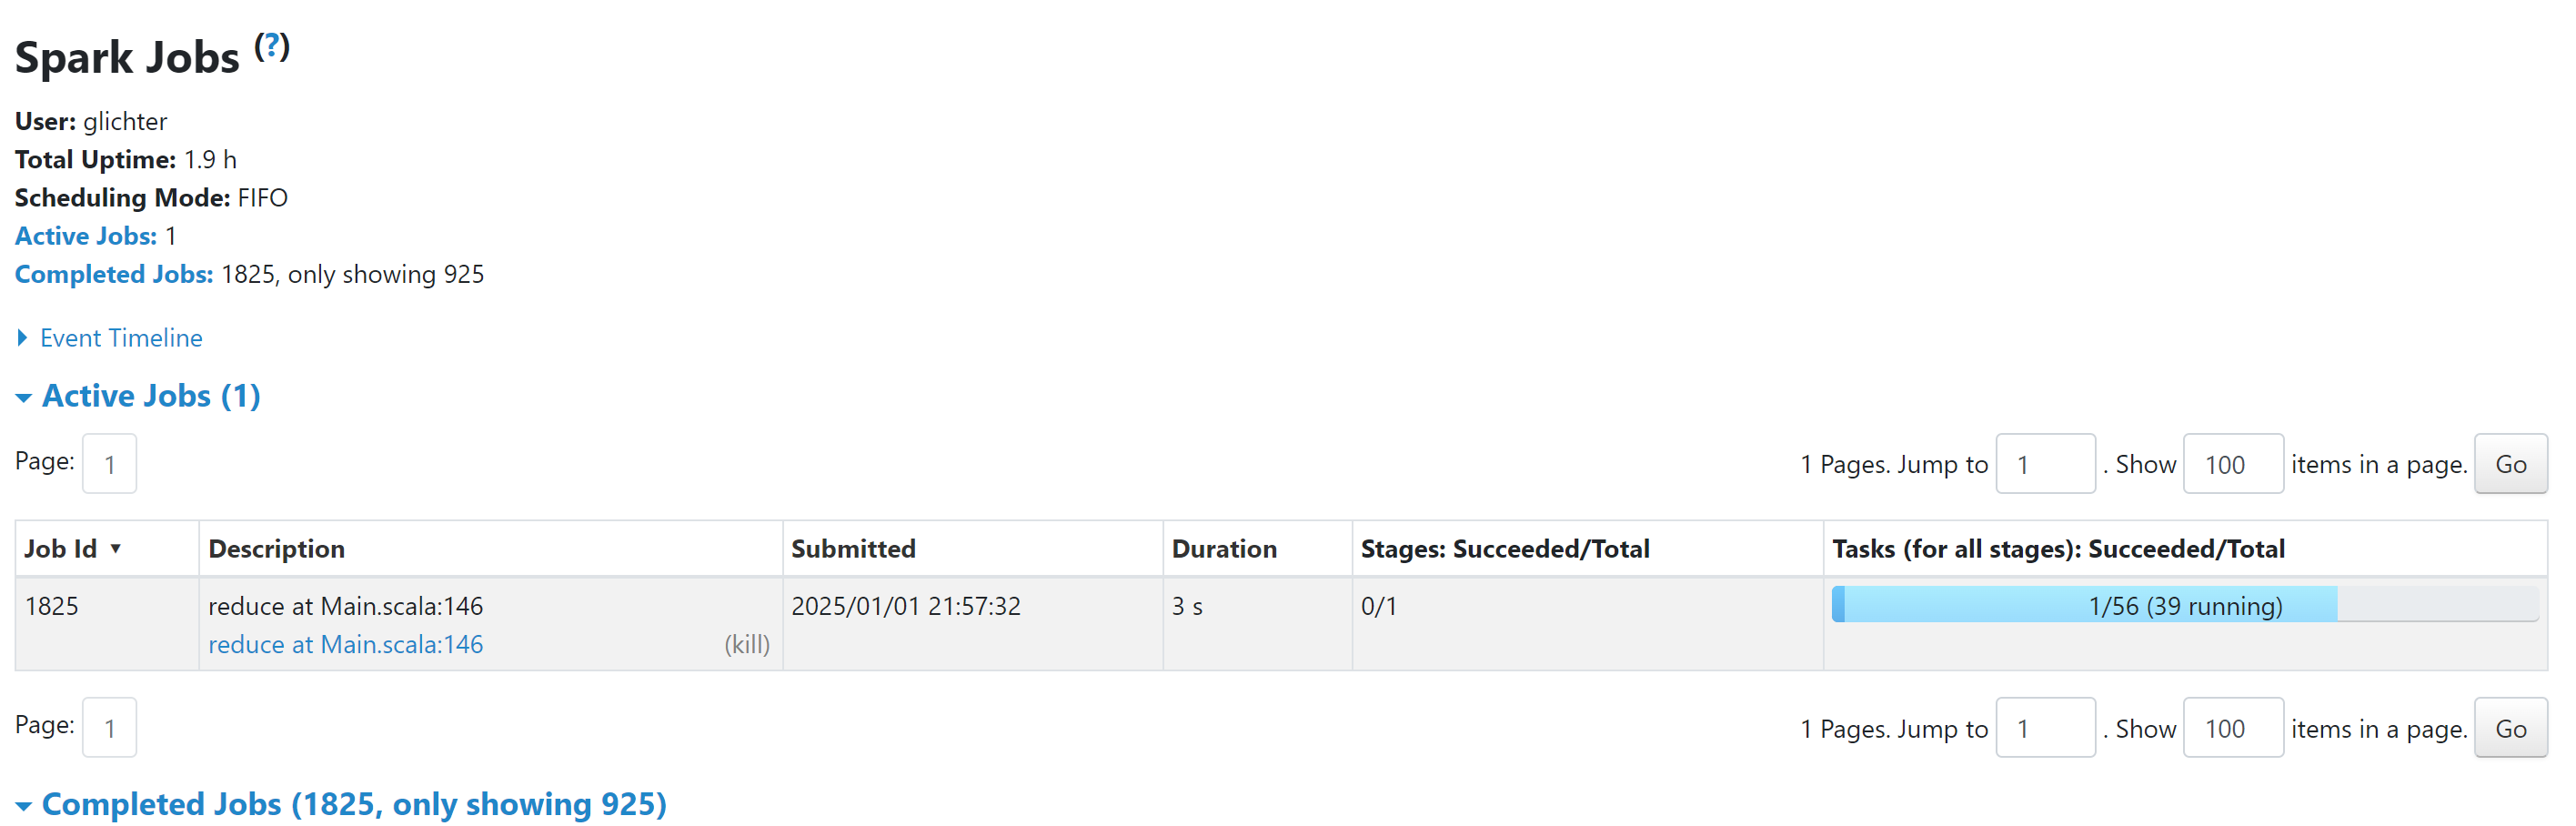
\includegraphics[width=\textwidth]{images/sparkscreenshot.png}
\end{figure}
\section{Questions}
\subsection{Have you persisted some of your intermediate results? Can you think of why persisting
	your data in memory may be helpful for this algorithm?}
Yes I persisted some of my intermediate results.
As mentioned in \ref{sec:design-decisions} I persisted the initial RDD resulted from reading the txt file.
I also persisted the RDD as a result from applying the gamma function to it.
As mentioned in class, apache spark lazily evaluates the operations done on the RDD's.
Which means that when an eager operation is invoked, all the previous lazy operations get applied to it's latest saved state.
When a lazy operation is invoked it just remembers the transformation and waits till an eager operation is called.
Consequently if its latest state is far away, it has to recompute a lot. This means that if a intermediate result is reused in multiple results derived from the intermediate results, it is beneficial to persist that intermediate result, to not recompute it in each result derived from it. Testing it with and without the persistance, showed that persisting the intermediate results yielded a big speedup. For example going from 4 minutes to 1 minute with a setup of K = 3 and Epsilon = 0,01
\subsection{
	In which parts of your implementation have you used partitioning? Did it help for
	performance? If so, why?
}
None, I did not make use of partitioning outside the default partitioning.
I figured since the dataset is not categorised or requires 'grouping' partitioning is not needed.
However, afterwards I thought perhaps I could have partitioned the dataset to group identical values together in the same partition to help with computing the GMM.
Perhaps instead of summing the results of the algorithm I could have applied the algorithm once to a value in the partition and then multiplied it by the amount of occurences of the value in the partition and then sum the results. Regardless, I did not trust my math skills enough to try this.
\subsection{
	Did you use RDDs, DataFrames or Datasets for your implementation? Why?
}
Truth be told I just followed the pseudocode where they used RDD's and did not know I had to 'defend' my choice afterwards. I thought I was free to use whichever I felt comfortable with using as the structure of the dataset did not prompt me to use a specific one.
I knew DataFrames and DataSets were more specialized for structured data, but since the dataset just had one column of numbers, I felt like all of the classes could be used.
Come to think of it, I did look up the other classes afterwards and thought it might have been better to use the DataFrames class, since it's more optimized than RDD's, according to the apache spark website.
\end{document}

